\chapter{Projektorganisation}

\section{Beteiligte Personen}
\label{sec:projektorganisation.BetroffenePersonen}

\textbf{Studierende:}\\
 Lukas Kuster \textit{kustl1@bfh.ch} \\
 Stefan K�ser \textit{kases1@bfh.ch}
 
\textbf{Betreuung:}\\
Dr. J�rgen Eckerle \textit{juergen.eckerle@bfh.ch}

\textbf{Experte:}\\
Dr. Federico Fl�ckiger	\textit{federico.flueckiger@bluewin.ch}


\section{Projektmeetings}
\label{sec:projektorganisation.Projektmeetings}

\begin{itemize}
\item Es findet ein Treffen mit dem Betreuer alle 1-2 Wochen statt.
\item Ein Treffen mit dem Experten findet am Anfang und am Ende der Arbeit statt, oder auf Wunsch des Experten.
\end{itemize}

\section{Dokumentation}
\label{sec:projektorganisation.Dokumentation}

Die Dokumentation soll sich am Aufbau und Inhalt des Berichts aus dem Projekt 2 anlehnen.
\begin{itemize}
\item Das Dokument beschr�nkt sich auf das Wesentliche.
\item Verwendete AI-Techniken werden erl�utert
\item Entscheidungen und deren Grundlagen sind dokumentiert.
\item Testberichte dokumentieren die durchgef�hrten Modultests. 
\item Klassendiagramme sollen einen oberfl�chlichen Detailierungsgrad haben, so dass das Wichtigste auf den ersten Blick sichtbar ist.
\item Anleitung zum Ausf�hren eines Spiels
\end{itemize}

\section{Abgabe}
\label{sec:projektorganisation.Abgabe}
Folgende Lieferobjekte werden am Ende der Arbeit abgegeben.
\begin{itemize}
\item Dokumentation
\item Sourcecode
\end{itemize}

\section{Zeitplan}
\label{sec:projektorganisation.Zeitplan}
Die Projektarbeit richtet sich nach folgendem Zeitplan:

\begin{figure}[bth]
\centering
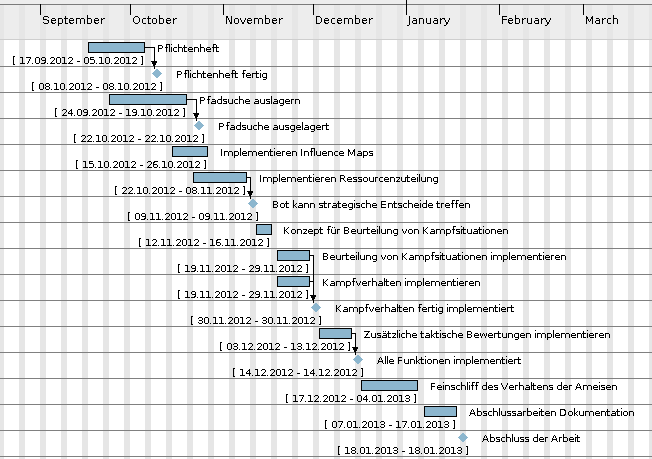
\includegraphics[width=0.9\textwidth]{bilder/gantt}
\caption{Projektablauf}
\label{fig:gantt}
\end{figure}
% \begin{tabular}{p{3cm}l}
%   \hline
%  \textbf{Datum} 			& \textbf{Arbeit}   \\
%  \hline
%  17.09.2012 	& Start der Arbeit \\
%  06.10.2012 	& Fertigstellung des Pflichtenhefts \\
%  19.10.2012 	& Framework zur Pfadsuche fertiggestellt \\
%  09.11.2012	& Bot kann strategische Entscheide treffen \\
%  16.11.2012	& Konzept f�r die Bewertung der Kampfformationen \\
%  30.11.2012	& Kampfverhalten implementiert \\
%  15.12.2012	& Programmierung gr�ssten Teils abgeschlossen \\
%  15-31.12.2012 & Korrekturen \& Feinschliff des Bots \\
%  11.01.2013	& Fertigstellung der Arbeit \\
%  11-18.01.2013		& Reserve \\
%  18.01.2013 	& Abgabe der Arbeit \\
%  tbd				 	& Verteidigung Bachelor Arbeit \\ 
% \end{tabular}
